\documentclass[11pt,letterpaper]{article}
\usepackage{anysize}
\usepackage{indentfirst}
\usepackage{sectsty}
\usepackage{amsmath}
\usepackage{hyperref}
\usepackage{graphicx}
\usepackage{chngpage}
\usepackage{enumerate}
\hypersetup{
	colorlinks=true, 
	linkcolor=blue, 
	urlcolor=blue, 
	pdfnewwindow=true, 
	citecolor=black
}
\urlstyle{same}
\linespread{1.2}

\begin{document}

\begin{titlepage}
    \vspace*{4cm}
    \begin{flushright}
    {\huge
        Project 2\\[5mm]
    }
    {\large
        CS325 | Spring 2015
     }
    \end{flushright}
\hrule
    \begin{flushright}
	by Group 2\\
	Vedanth Narayanan\\
	Jonathan Merrill\\
	Tracie Lee\\
    \vfill
	\today\\
    \end{flushright}
\end{titlepage}

\raggedright

\section*{Dynamic Programming Table}

\section*{Algorithm Pseudocode}
\begin{verbatim}
-- Divide and Conquer --

Define changeslowhelper(currency[], amount)
    // currency = array of coin denominations
    // amount = int, total amount we're making change for
    
    if amount == 0
        return 0
    for each coin in currency
        if coin == amount
            return [coin]
			
    for i to amount/2
        temp.extend(changeslowhelper(currency, i))
        temp.extend(changeslowhelper(currency, amount - 1))
        numCoins = length of temp
		
        if numCoins < minCoins
            coins = temp
	
    return coins
	
Define changeslow(currency[], amount)
    coins = changeslowhelper(currency[], amount)
	
    for each coin in currency
        result.append(coins.count(coin))
	
    return result
	
===================================================================================
===================================================================================
-- Greedy --

Define changegreedy (currency[], amount)
    int num
	
    for i to currency.length
		
        if currency[i] <= amount
            num = amount / currency[i]
            numArray[i] = numArray[i] + num
            total = total + num
            amount -= num * currency[i]
	
    numArray.append(total)  // sending the total through on the end of the array
                            // then we'll strip it off in the print function
    return numArray
    
===================================================================================
===================================================================================
-- Dynamic Programming --

Define changedp (currency[], amount)


\end{verbatim}

\section*{Dynamic Programming Induction Proof}
	Proof by Induction:
\begin{itemize}
	\item \textbf{Base Case}\\
	T[0] = 0. This is true because for 0 cents, the optimal number of coins used is 0.
	\item \textbf{Inductive Hypothesis}\\
	We assume that for some arbitrary value 'k', T[k] is the minimum number of coins used to make change for k cents. This also assumes that T[p] is correct, where p is any value less than or equal to k, due to the nature of the problem.
	\item \textbf{Inductive Step}\\
	We must now prove that T[k+1] is also correct:\\
	\hspace{15pt}Since:\\ 
	\hspace{30pt}T[k+1] = T[(k+1) - i] + 1; where i is some value less than or equal to k\\
	\hspace{15pt}Then:\\
	\hspace{30pt}T[k+1] = T[p] + 1; where p is some value less than or equal to k\\
	Since we know T[p] is the correct number of coins used for p cents, T[k+1] must also be the correct number of coins used for k+1 cents.
\end{itemize}	 
\section*{Questions}
\begin{enumerate}
	\item Suppose V = [1, 5, 10, 25, 50]. For each integer value of A in [2010, 2015, 2020, ..., 2200] determine the number of coins that changegreedy and changedp requires. You can attempt to run changeslow however if it takes too long you can select smaller values of A and also run the other algorithms on the values. Plot the number of coins as a function of A for each algorithm. How do the approaches compare?
	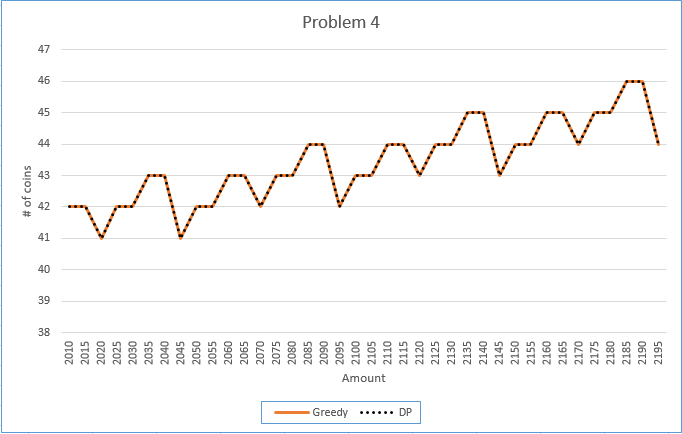
\includegraphics[width=6in]{p4.png}
	As you can see, both algorithms are identical in the results produced for V = [1,5,10,25,50].
	\item Suppose V1 = [1, 2, 6, 12, 24, 48, 60] and V2 = [1, 6, 13, 37, 150]. For each integer value of A in [2000, 2001, 2002, ..., 2200] determine the number of coins that changegreedy and changedp requires. If your algorithms run too fast try [10000, 10001, 10003, ..., 10100]. You can attempt to run changeslow however if it takes too long you can select smaller values of A and also run all three algorithms on the values. Plot the number of coins as a function of A for each algorithm. How do the approaches compare?
	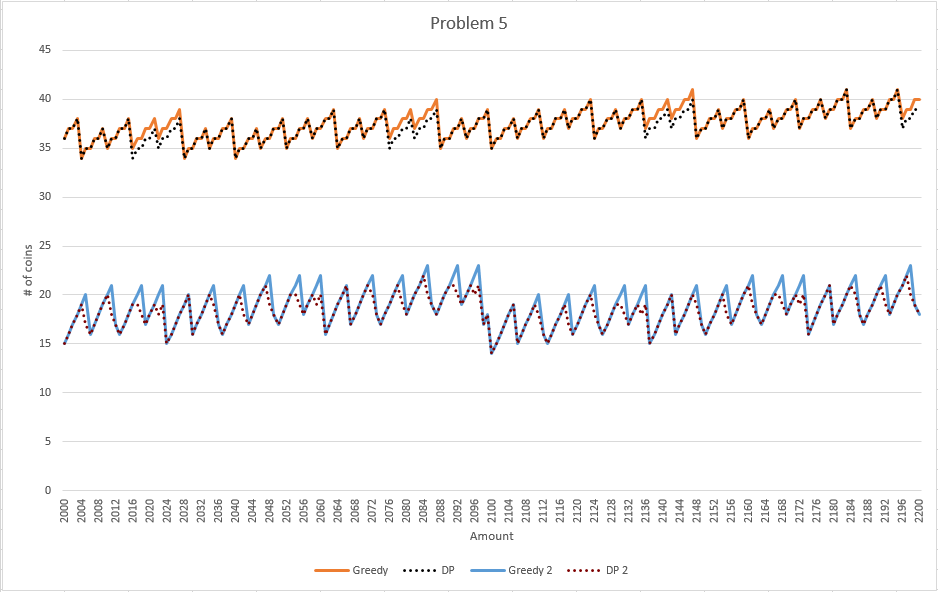
\includegraphics[width=6in]{p5.png}\\
	For some values in the Dynamic Programming algorithm, more minimized results are returned in comparison to the greedy algorithm. This is true for both V = [1, 2, 6, 12, 24, 48, 60] and V = [1, 6, 13, 37, 150].
	\item Suppose V = [1, 2, 4, 6, 8, 10, 12, ..., 30]. For each integer value of A in [2000, 2001, 2002, ..., 2200] determine the number of coins that changegreedy and changedp requires. You can attempt to run changeslow however if it takes too long you can select smaller values of A and also run all three algorithms on the values. Plot the number of coins as a function of A for each algorithm.
	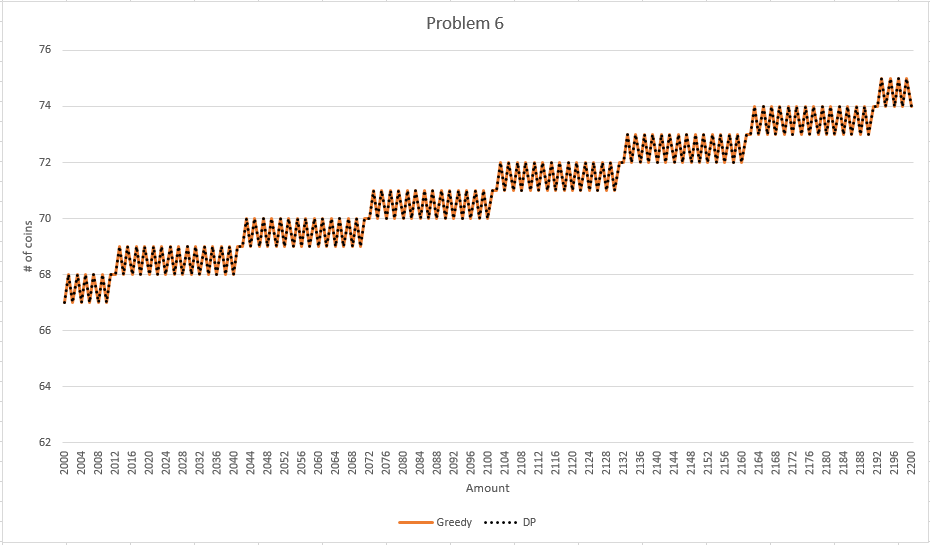
\includegraphics[width=5.5in]{p6.png}\\
	As you can see, both algorithms are identical in the results produced for V = [1, 2, 4, 6, 8, 10, 12, ..., 30].
	\item For the above situations, determine (experimentally) the running times of the algorithms by fitting trend lines to the data or analyzing the log-log plot. Graph the running time as a function of A. Compare the running times of the different algorithms.\\
	\textbf{Problem 4}\\
	\hskip-1.0cm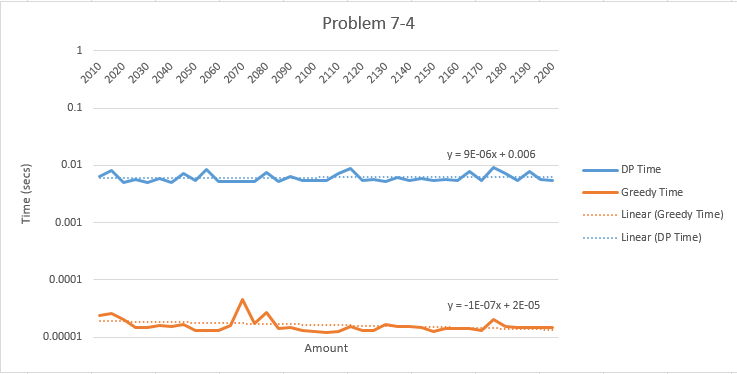
\includegraphics[width=6.5in]{p7-4.png}\\
	\textbf{Problem 5}\\
	\hskip-1.0cm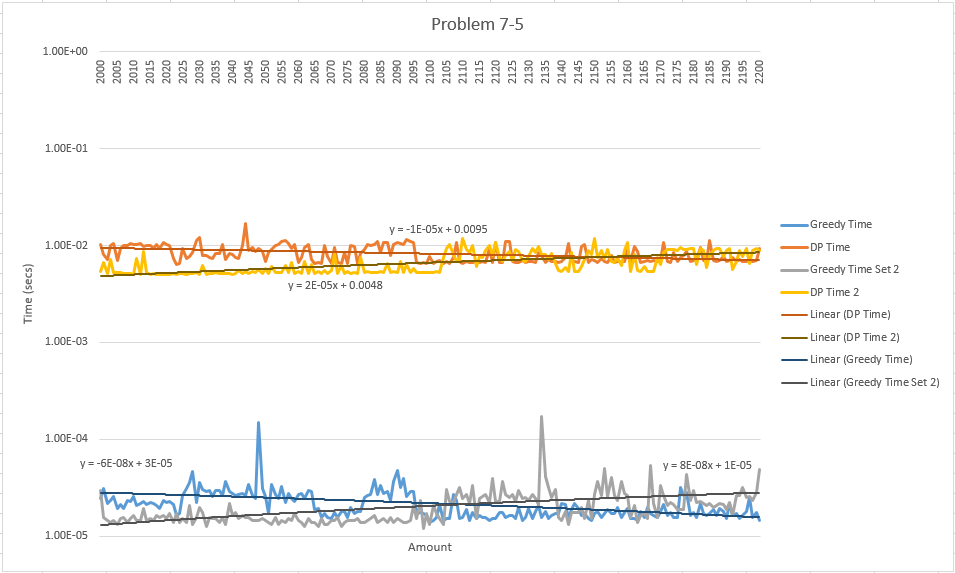
\includegraphics[width=6.5in]{p7-5.png}\\
	\textbf{Problem 6}\\
	\hskip-1.0cm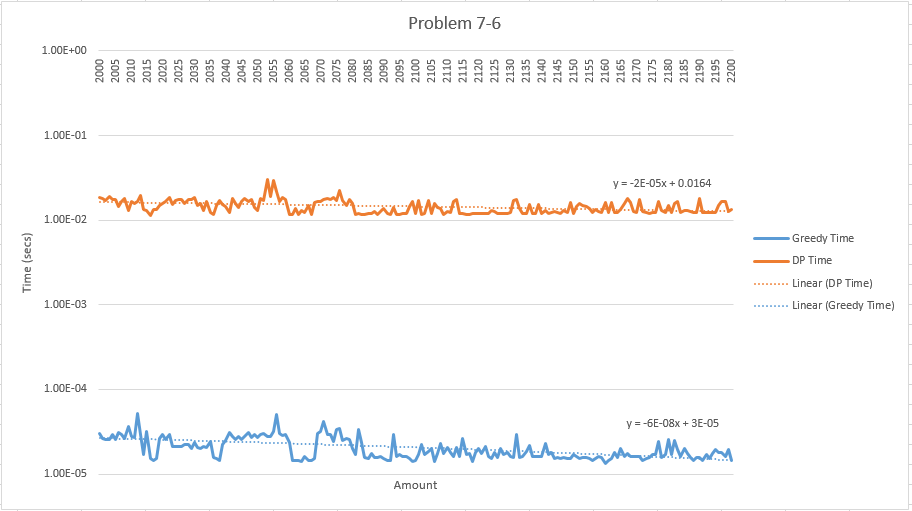
\includegraphics[width=6.5in]{p7-6.png}
	
	
	\item Use the data from questions 4-6 and any new data you have generated. Plot running times as a function of number of denominations (i.e. V=[1, 10, 25, 50] has four different denominations so n=4). Does the size of n influence the running times of any of the algorithms?
	\item Suppose you are living in a country where coins have values that are powers of p, V = [$p^0$, $p^1$, $p^2$, ... , $p^n$]. How do you think the dynamic programming and greedy approaches would compare? Explain.
\end{enumerate}

\end{document}
